% Deve resumir o experimento, os resultados e a discussão (comentários)
% e incluir opiniões do grupo e propostas futuras para o experimento
%Descrição do hardware
%Descrição do software
%\cite{Advpdf}
%\cite{thepdf}
%\cite{dsl}

\subsection{Estruturas}\label{struct}

\subsubsection{Arquitetura}\label{arq}

No intuito de manter o jogo compatível com qualquer sistema operacional, foi decidido centralizar as inclusões de bibliotecas em um único arquivo. Para essa função foi criado o arquivo \textit{"defines.h"}, que é responsável por reconhecer o sistema em que esta sendo compilado e incluir os devidos \textit{headers}.

\begin{lstlisting}[language=C++,title=\textit{defines.h},firstnumber=5,numbers=none]
#if defined (__APPLE__) || defined (MACOSX) /*MAC OS*/
    #include <GLUT/glut.h>
#else
    #ifdef _WIN32                           /* Windows */
    	#define WIN32_LEAN_AND_MEAN
        #include <glee.h>
        #include <gl/gl.h>
		#include <gl/glut.h>
        #include <windows.h>
        #define sleep(x) Sleep(x)
    #else                                   /*Linux*/
    	#include <cstdarg>
    	#include <unistd.h>
        #include <GL/gl.h>
        #include <GL/glut.h>
        #include <GL/glu.h>
        #define Sleep(x) usleep(x<1000000?10000+300*x:x)
    #endif
#endif
\end{lstlisting}

No trecho mostrado acima, podemos ver como o programa reconhece em qual sistema esta sendo compilado e em qual endereço irá procurar pelas bibliotecas. A decisão é tomada de forma bem simples e objetiva, buscando apenas saber se as definições \textbf{MACOSX} ou \textbf{\_WIN32} existem. Com estas duas definições é suficiente para dividir entre os três sistemas operacionais que o programa se propõe a dar suporte. 

Porém este não é o único problema enfrentado quando se trata de um programa multiplataforma, mas também existem as dificuldades com a própria compilação.

Visando isso, foi feito um arquivo \textit{makefile} que procede com teste semelhante ao feito no \textit{defines.h} para verificar em que sistema se encontra e assim efetuar os links corretamente. Um trecho do \textit{makefile} pode ser observado a seguir:

\begin{lstlisting}[language=make,title=\textit{Makefile},firstnumber=8,numbers=none]
UNAME = $(shell uname)
ifeq ($(UNAME),Linux) # Linux OS
	GLFLAGS = -lglut -lglui -lGLU -lGL 
	else
	ifeq ($(UNAME),Darwin) # MAC OS X
		GLFLAGS = -framework OpenGL -framework GLUT
	else #Windows
		GLFLAGS = -lopengl32 -lglu32 -lglut32 -lglee
	endif
endif
\end{lstlisting}


%-----------------------------------------------------------------------------------------------------------------
Na seção desenvolvimento deve ser respondidas as seguintes perguntas:
 
	\begin{itemize}
		\item Estrutura do Programa: Qual a estruturação/arquitetura do Programa?
	 	\item Qual é o procedimento para a execução do programa? 
	 	\item Quais artefatos são necessários para a execução do programa?
	 	\item Quais os problemas técnicos enfrentados no desenvolvimento do programa?
	 	\item Como os pontos relacionados à disciplina foram abordados no problema? Quais as lições aprendidas? Quais as principais dificuldades?
	 	\item Quais elementos teóricos abordado na disciplina foram implementados no programa?
	 	\item Quais adaptações, extensões, bibliotecas externas, foram necessários para a solução do problema?
	 	\item Caso use parte de códigos disponibilizados na Web, colocar referência \footnote{A home-page de onde tirei
este material:\url{http://en.wikibooks.org/wiki/LaTeX}.Estou formatando para \LaTeX apenas para os estudantes irem se orientando de como e o quê escrever.Assim, me isento de responsabilidade sobre o conteúdo deste texto. Dúvidas: carla(rocha.carla@gmail.com)}
	\end{itemize}
	
	As Figuras são simplesmente inseridas como mostrado na Fig. \ref{Fig1}
	
\begin{figure}[ht]
  \centering
  %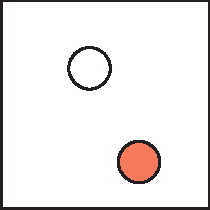
\includegraphics[width=5cm]{figs/samplefigure}
   \caption{Arquitetura do Programa.}
  \label{Fig1}
\end{figure}
 
\subsection{Artefatos}
\label{SebSec:Artefatos}
Os artefatos entregues devem ser documentados no relatório:
\begin{itemize}
\item Arquivos contidos no programa. Lista dos nomes dos arquivos, assim como a extensão dos arquivo
\item Aquivo README, com instruções de uso do software desenvolvido e necessidades técnicas para a execução do programa
\item Arquivos de entrada/saída, caso necessário.
\end{itemize}

